\documentclass[tikz]{standalone}
\usepackage{tkz-graph}
\usepackage{amsmath,amssymb}
\usepackage{xcolor}
\usetikzlibrary{calc}
\usetikzlibrary{positioning}
\usetikzlibrary{shapes.geometric}

% https://latexdraw.com/tikz-shape-diamond/
\begin{document}

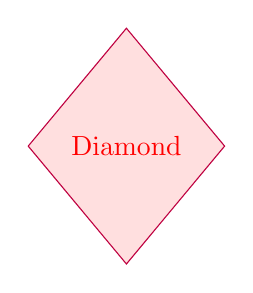
\begin{tikzpicture}
	\node [draw=purple, diamond, text=red, fill=pink!50, minimum width = 2.5cm, minimum height=3cm] (d) at (0,0)  {Diamond};
\end{tikzpicture}

\end{document}
